\documentclass[xcolor=dvipsnames, aspectratio=169]{beamer}
\usepackage[utf8]{inputenc}
\usepackage[T1]{fontenc}
\usepackage[english]{babel}
\usetheme{Northeastern}
\usepackage{booktabs}
\usepackage{amsmath}
\usepackage{amssymb}
\usepackage{caption}
\usepackage{subcaption}
\usepackage{cancel}
\usepackage{algorithm}
\usepackage{hyperref}
\usepackage[noend]{algpseudocode}
\usepackage{standalone}
\usepackage{tikz}
\usepackage{wrapfig}
\usetikzlibrary{shapes.geometric,positioning,arrows.meta}
\graphicspath{{media}, {images}}
\usepackage{pgfkeys}
\usepackage[most]{tcolorbox}
\tcbuselibrary{minted}
\usepackage{codebox}

% NU colors
% from https://brand.northeastern.edu/visual-design/color/
\definecolor{NURed}{RGB}{200, 16, 46}
\definecolor{NUGold}{RGB}{164, 128, 74}
\definecolor{NUOrange001}{RGB}{255,175,128}
\definecolor{NUOrange002}{RGB}{255,153,102}
\definecolor{NUOrange003}{RGB}{255,133,79}
\definecolor{NUOrange004}{RGB}{229,98,28}
\definecolor{NUOrange005}{RGB}{187,65,0}
\definecolor{NUYellow001}{RGB}{255,255,165}
\definecolor{NUYellow002}{RGB}{255,213,128}
\definecolor{NUYellow003}{RGB}{255,196,75}
\definecolor{NUYellow004}{RGB}{255,184,56}
\definecolor{NUYellow005}{RGB}{226,168,85}
\definecolor{NUGreen001}{RGB}{189,233,201}
\definecolor{NUGreen002}{RGB}{152,209,181}
\definecolor{NUGreen003}{RGB}{96,159,128}
\definecolor{NUGreen004}{RGB}{2,89,68}
\definecolor{NUGreen005}{RGB}{26,69,56}
\definecolor{NUBlue001}{RGB}{198,239,252}
\definecolor{NUBlue002}{RGB}{160,224,239}
\definecolor{NUBlue003}{RGB}{98,182,208}
\definecolor{NUBlue004}{RGB}{43,116,150}
\definecolor{NUBlue005}{RGB}{12,51,84}

% Define colors outside of the scope of beamer themes
\newcommand{\defaultcolorheading}{NUGreen003}

% highlighted 'headings'
\newcommand{\colorheading}[1]{\textcolor{\defaultcolorheading}{\LARGE #1}}
\newcommand{\colorcaption}[1]{\textcolor{\defaultcolorheading}{\footnotesize #1}}

% Section frame, no table of contents displayed
\newcommand{\sectionframe}[2]{
  {
    \setbeamercolor{background canvas}{bg=white}
    \begin{frame}[noframenumbering, plain]
      \begin{minipage}{0.475\textwidth}
        \centering
        {\usebeamerfont{titlelike}\usebeamercolor[fg]{structure}\huge #1}
      \end{minipage}
      \hfill
      \begin{minipage}{0.45\textwidth}
        \centering
        {#2}
      \end{minipage}
    \end{frame}
  }
}

% Section frame with table of contents
\newcommand{\sectioncontentsframe}[2]{
  {
    \setbeamercolor{background canvas}{bg=white}
    \begin{frame}[noframenumbering, plain]
      \begin{center}
      \begin{minipage}{0.475\textwidth}
        \centering
        {\usebeamerfont{titlelike}\usebeamercolor[fg]{structure}\huge #1}
        \vskip2em
        \setbeamercolor{normal text}{fg=black}
        \setbeamertemplate{subsection in toc}{\leavevmode\leftskip=1.2em$\bullet$\hskip0.25em\inserttocsubsection\par}
        \tableofcontents[currentsection, sectionstyle=hide, subsubsectionstyle=hide]
      \end{minipage}
      \hfill
      \begin{minipage}{0.475\textwidth}
        \centering
        {#2}
      \end{minipage}
      \end{center}
    \end{frame}
  }
}

\newtcolorbox{alertbox}[1][]{enhanced,
  before skip=2mm,after skip=3mm,
  boxrule=0.4pt,left=5mm,right=2mm,top=1mm,bottom=1mm,
  colback=NUYellow001,
  colframe=NUYellow003,
  sharp corners,rounded corners=southeast,arc is angular,arc=3mm,
  underlay={%
    \path[fill=NUYellow005] ([yshift=3mm]interior.south east)--++(-0.4,-0.1)--++(0.1,-0.2);
    \path[draw=tcbcolframe,shorten <=-0.05mm,shorten >=-0.05mm] ([yshift=3mm]interior.south east)--++(-0.4,-0.1)--++(0.1,-0.2);
    \path[fill=NUYellow005,draw=none] (interior.south west) rectangle node[white]{\Huge\bfseries !} ([xshift=4mm]interior.north west);
  },
  drop fuzzy shadow,#1}

\newtcolorbox{infobox}[1][]{enhanced,
  before skip=2mm,after skip=3mm,
  boxrule=0.4pt,left=5mm,right=2mm,top=1mm,bottom=1mm,
  colback=NUGreen001,
  colframe=NUGreen003,
  sharp corners,rounded corners=southeast,arc is angular,arc=3mm,
  underlay={%
    \path[fill=NUGreen003] ([yshift=3mm]interior.south east)--++(-0.4,-0.1)--++(0.1,-0.2);
    \path[draw=tcbcolframe,shorten <=-0.05mm,shorten >=-0.05mm] ([yshift=3mm]interior.south east)--++(-0.4,-0.1)--++(0.1,-0.2);
    \path[fill=NUGreen003,draw=none] (interior.south west) rectangle node[white]{\Huge\bfseries i} ([xshift=4mm]interior.north west);
  },
  drop fuzzy shadow,#1}

% Pygments theme
\newcommand{\PygmentsStyle}{colorful}

% default color for boxes
\newcommand{\CodeBoxFgColor}{NUGreen005}
\newcommand{\CodeBoxBgColor}{NUGreen001!10}
\newcommand{\CodeHighlightColor}{NUOrange004!20}

% Boxes to display code
\newtcblisting[auto counter]{codeboxtc}[4]{%
  title=#2,
  listing only,
  %minted style=\PygmentsStyle,
  minted language=#1,
  boxsep=0.25mm,
  left=1mm,
  right=1mm,
  top=1mm,
  bottom=1mm,
  colback=\CodeBoxBgColor,
  colbacktitle=\CodeBoxFgColor,
  colframe=\CodeBoxFgColor,
  fonttitle=\scriptsize,
  minted options={autogobble,fontsize=\small, fontfamily=courier,
    breaklines=true, linenos, #4},
  #3
}

\newtcbinputlisting[auto counter]{\codeinput}[5]{%
  title=#2,
  listing only,
  %minted style=\PygmentsStyle,
  minted language=#1,
  boxsep=0.25mm,
  left=1mm,
  right=1mm,
  top=1mm,
  bottom=1mm,
  colback=\CodeBoxBgColor,
  colbacktitle=\CodeBoxFgColor,
  colframe=\CodeBoxFgColor,
  fonttitle=\scriptsize,
  minted options={autogobble,fontsize=\small, fontfamily=courier,
    breaklines=true, highlightcolor=\CodeHighlightColor, linenos, highlightlines=#4},
  listing file=#5,
  #3
}

\newcommand{\BeamerShowCode}[3]{%
  \pgfkeys{
    /highlight lines/.initial=4,
    /highlight lines/.get=\codehighlight,
    /highlight lines/.store in=\codehighlight,
    /extra tcb options/.initial=\empty,
    /listing file/.initial=file.cpp,
    /minipage width/.initial=1.0\textwidth,
    /box scale/.initial=1,
    /language/.initial=cpp,
  }
  \pgfkeys{#1}
  \scalebox{\pgfkeysvalueof{/box scale}}{
    \begin{minipage}{\pgfkeysvalueof{/minipage width}}
      \centering
      \codeinput{\pgfkeysvalueof{/language}}{#2}
          {\pgfkeysvalueof{/extra tcb options}}{#3}{\pgfkeysvalueof{/listing
          file}}
    \end{minipage}%
  }
}
\graphicspath{{media}, {images}}
\titlegraphic{
\includegraphics[width=0.4\paperwidth]{northeastern}}

\title{Navigating Programming Education in AI Age}
\author{Gunar Schirner, Fatema Nafa, Muhammad Salman}
\institute{Embedded Systems Laboratory (ESL)\\
  Electrical And Computer Engineering\\
  Northeastern University\\
  Boston MA, USA}
\newcommand{\footername}{AI in Programming Education}

\begin{document}

\begin{frame}[plain]
  \titlepage
\end{frame}

\begin{frame}{Outline}
  \tableofcontents[part=1]
  \tableofcontents[hideallsubsections, part=2]
  \tableofcontents[hideallsubsections, part=3]
  \tableofcontents[hideallsubsections, part=4]
  \tableofcontents[hideallsubsections, part=5]
\end{frame}

\part[Introduction]{Introduction}
\section{Introduction}

\begin{frame}{Workshop Information}
  \begin{columns}
    \begin{column}{0.58\textwidth}
      \textbf{Overview \& Objectives}
      \begin{itemize}\small
        \item Workshop for instructors teaching programming courses
        \item Explore AI's shift from syntax to system design
        \item Practice multiple levels of AI programming assistance
        \item Design meaningful classroom activities using AI
        \item Shift focus to higher-level design thinking
      \end{itemize}
      
      \textbf{Logistics \& Agenda}
      \begin{itemize}\small
        \item \textbf{Duration:} 1 hour, \textbf{Format:} Interactive
        \item \textbf{Requirements:} Programming knowledge, laptop
        \item AI in programming education [10 min]
        \item AI assistance levels exploration [15 min]
        \item Hands-on activity design [20 min]
        \item Discussion \& reflection [15 min]
      \end{itemize}
    \end{column}
    
    \begin{column}{0.38\textwidth}
      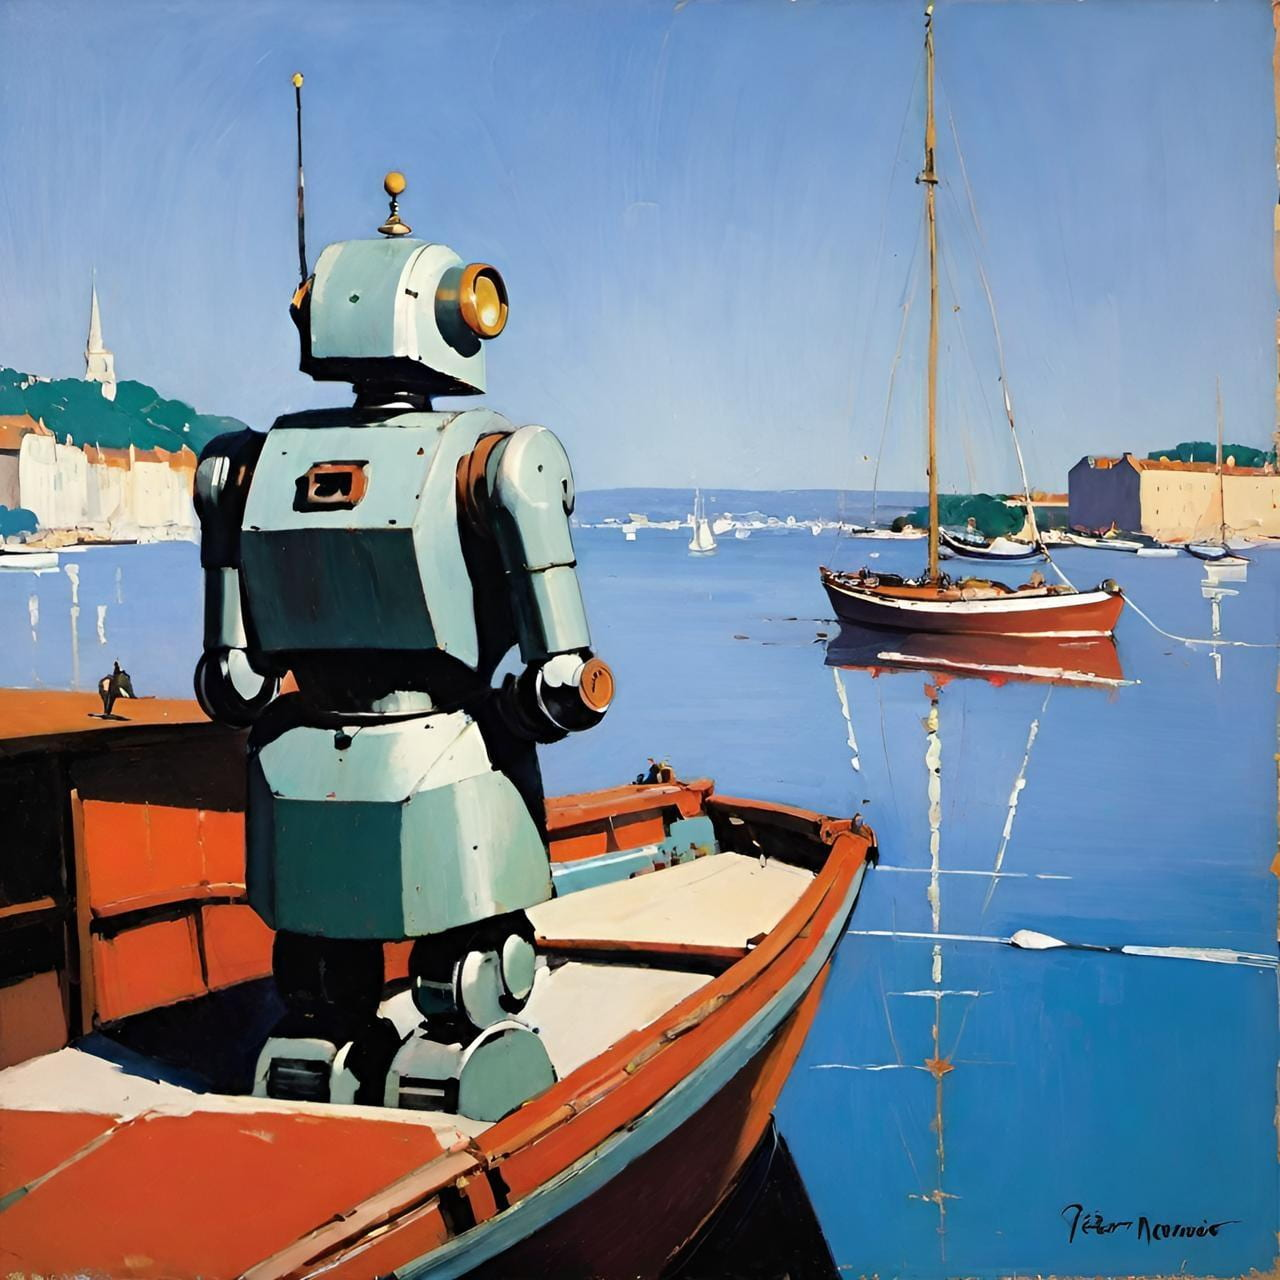
\includegraphics[width=\textwidth]{images/ai_programming.jpeg}
      \vspace{0.2cm}
      \small\centerline{AI enhancing programming education}
    \end{column}
  \end{columns}
\end{frame}

\section{Increasing Abstraction in Programming}

\begin{frame}{Evolution of Programming Abstractions}
  \begin{columns}
    \begin{column}{0.6\textwidth}
      \begin{itemize}
        \item Always moving toward higher levels of abstraction
        \item Increase managable system complex with less code
        \item Shift from implementation to system design
        \item Standard abstraction concerns:
          \begin{itemize}
            \item Performance
            \item Loss of control over implementation details
          \end{itemize}
        \item Abstractions dominate as compilers improve
        \item Example: Assembly only for utmost performance-critical code
          \begin{itemize}
            \item Where human expertise exceeds compiler optimization (for new HW features)
          \end{itemize}
      \end{itemize}
    \end{column}
    
    \begin{column}{0.4\textwidth}
      \centering
      \begin{tikzpicture}[scale=0.9]
        % Pyramid layers
        \fill[blue!20] (0,0) -- (4,0) -- (3.5,0.8) -- (0.5,0.8) -- cycle;
        \fill[blue!30] (0.5,0.8) -- (3.5,0.8) -- (3,1.6) -- (1,1.6) -- cycle;
        \fill[blue!40] (1,1.6) -- (3,1.6) -- (2.5,2.4) -- (1.5,2.4) -- cycle;
        \fill[blue!50] (1.5,2.4) -- (2.5,2.4) -- (2.25,3.0) -- (1.75,3.0) -- cycle;
        \fill[blue!60] (1.75,3.0) -- (2.25,3.0) -- (2,3.5) -- cycle;
        
        % Labels
        \node[align=center] at (2,0.4) {\small Machine Code};
        \node[align=center] at (2,1.2) {\small Assembly};
        \node[align=center] at (2,2.0) {\small C/C++};
        \node[align=center] at (2,2.7) {\small Python};
        \node[align=center] at (2,3.3) {\small Domain-specific};
        
        % Arrow and properties
        \draw[-{Stealth[scale=0.8]}] (4.5,0) -- (4.5,3.5);
        
        % Text for properties - right side of arrow
        \node[anchor=west, align=left, font=\tiny] at (4.6,3.2) {Higher abstraction};
        \node[anchor=west, align=left, font=\tiny] at (4.6,2.8) {Less code};
        \node[anchor=west, align=left, font=\tiny] at (4.6,2.4) {Design focus};
        
        \node[anchor=west, align=left, font=\tiny] at (4.6,1.2) {More control};
        \node[anchor=west, align=left, font=\tiny] at (4.6,0.8) {Performance};
        \node[anchor=west, align=left, font=\tiny] at (4.6,0.4) {Lower abstraction};
      \end{tikzpicture}
    \end{column}
  \end{columns}
  
  \begin{alertbox}
    \begin{itemize}
      \item With Generative AI, natural language becomes a new abstraction level
      \item Allows specifying what a program should do without syntax constraints
    \end{itemize}
  \end{alertbox}
\end{frame}


\begin{frame}{Paradigm Shift in Programming}
  \begin{columns}
    \begin{column}{0.6\textwidth}
      \begin{itemize}
        \item GenAI becomes peer programmer (collaborator)
          \begin{itemize}
            \item Generating simple scripts with a few sentences
            \item Reviewing, analyzing, and suggesting improvements
            \item Code completion, repeating, and expanding code patterns
            \item Developing complete projects across multiple files
          \end{itemize}
        \item Eases access to: languages, libraries and domains
        \item Led by human creativity, intuition, experience, and problem-solving
        \item Limited to what it abstracted from training data
        \item AI cannot build your custom, novel, high-impact project for you
        \begin{itemize}
            \item Can help build it faster and with less effort
            \item Helps focus on system design rather than implementation details
          \end{itemize}
      \end{itemize}
    
    \end{column}
    
    \begin{column}{0.4\textwidth}
      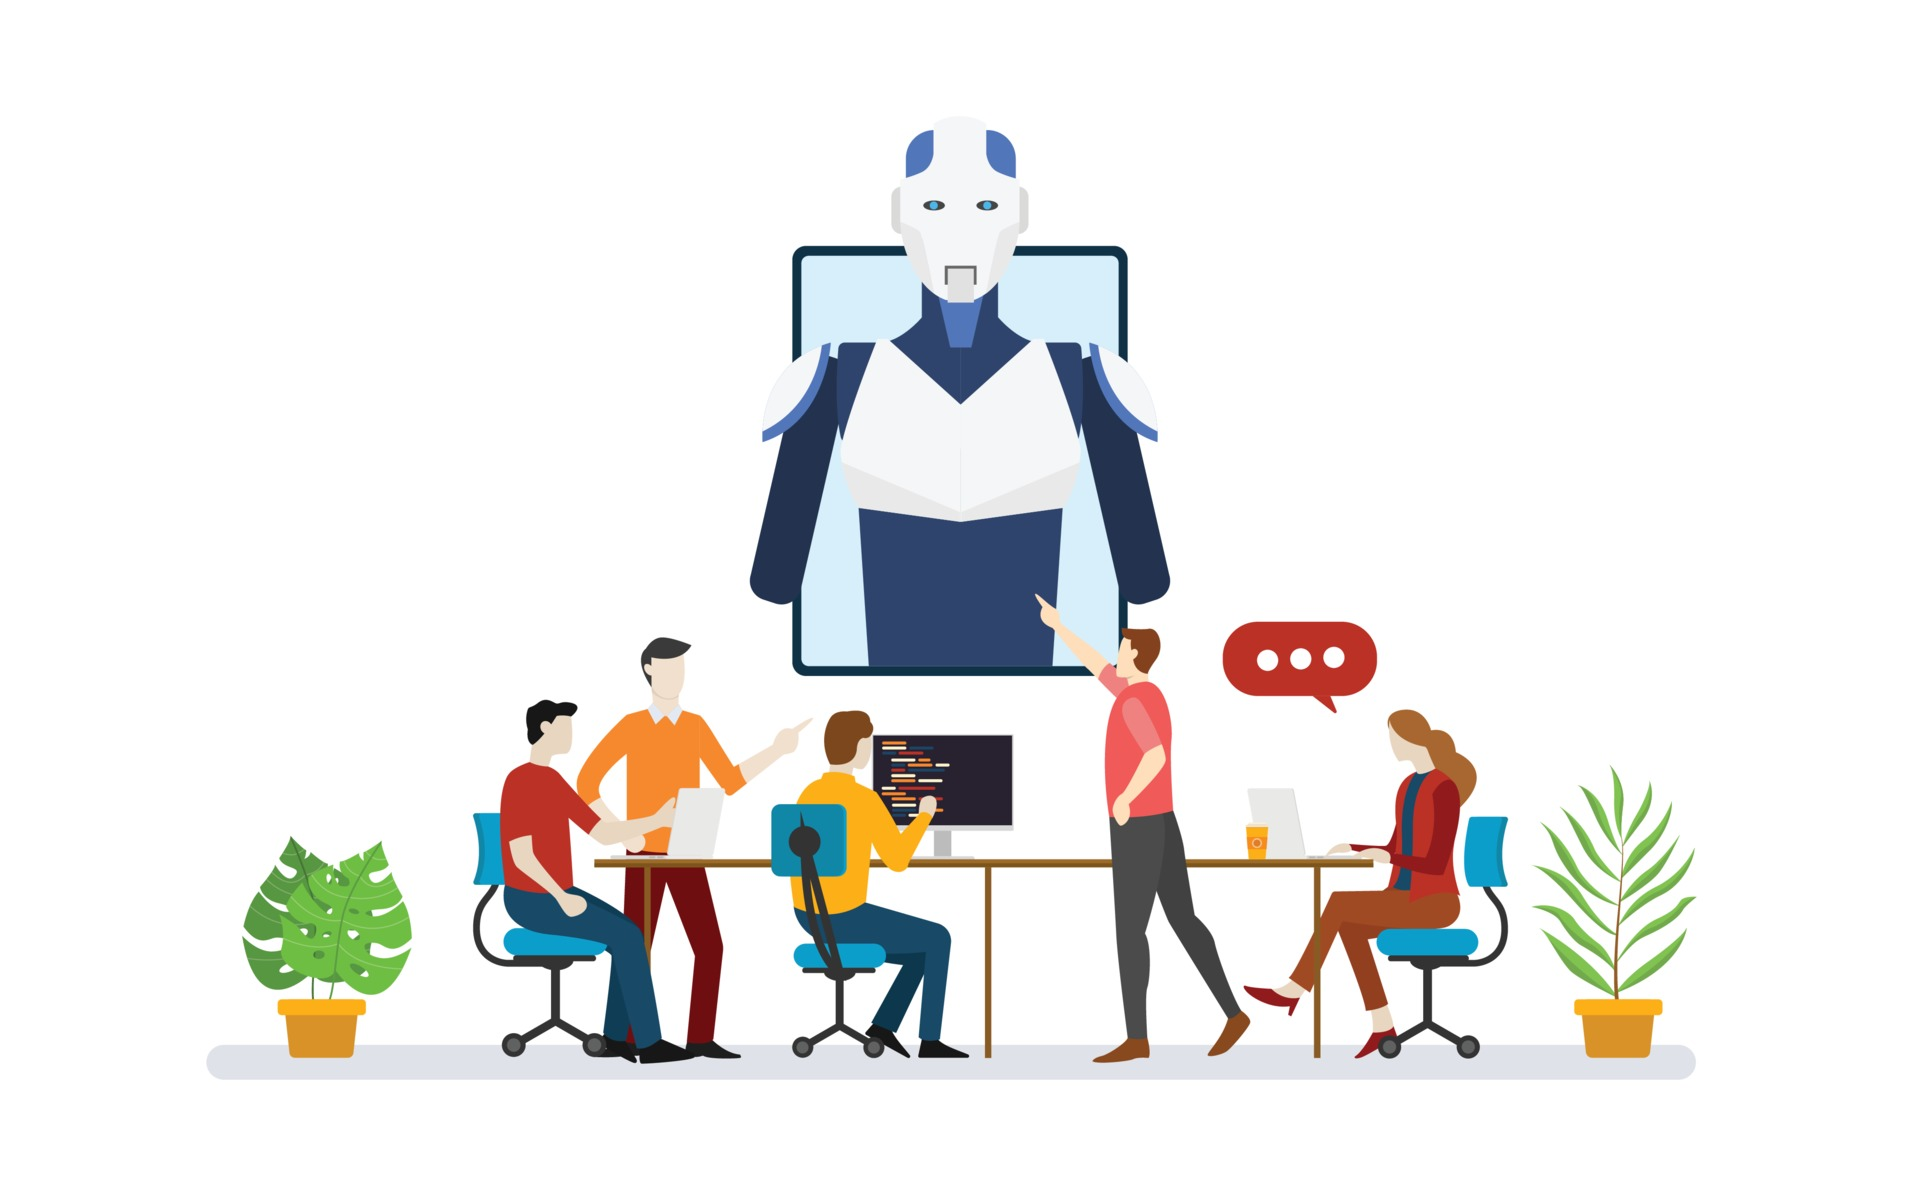
\includegraphics[width=\textwidth]{images/376_generated.jpg}
      %TODO make into caption, citation and bibtex
      \tiny\centerline{Image: "AI Robot Team Developer" by Vecteezy}
      \tiny\centerline{\url{www.vecteezy.com/vector-art/3216651}}
    \end{column}
  \end{columns}
\end{frame}


\begin{frame}{Changing Role of a Programmer}
  \begin{itemize}
    \item Focus shifts from \textbf{syntax and implementation mechanics} to \textbf{design, clear vision and intent}
    \item From \textbf{individual contributor} to \textbf{project team lead} where AI is a \textbf{collaborative team member}
    \item Enables larger-scale, impactful projects through AI assistance
    \item Still needs to understand the entire stack to evaluate suggestions and spot issues
  \end{itemize}
  
  %TODO: add image of a pilot and autopilot
  \begin{alertbox}
    Comparison with aircraft autopilot:
    \begin{itemize}
      \item Autopilot helps with low-level tasks, but pilot remains in control
      \item Pilot must understand entire aircraft systems to spot and fix issues
    \end{itemize}
  \end{alertbox}
  %TODO: alertbox is not the right thing, need a question box
  \begin{alertbox}
    \begin{itemize}
      \item How do we ensure students understand the underlying technology details?
      \item How do we guide them to become technology leaders?
    \end{itemize}
  \end{alertbox}
\end{frame}


\part[AI Programming Assistance]{AI Programming Assistance}
\section{Overview of Assistance Levels}

\begin{frame}{Four Levels of AI Programming Assistance}
  We'll explore four examples of AI programming assistance, with increasing complexity and integration:
  
  \begin{enumerate}
    \item \textbf{Auxiliary Code Generation}\\
    One-shot generation of scripts beyond course focus
    
    \item \textbf{Code Review and Improvement}\\
    Analyze, debug, and enhance existing code with AI
    
    \item \textbf{Copilot Integration in VS Code}\\
    Contextual code completion with GitHub Copilot
    
    \item \textbf{Agent Mode for Complex Projects}\\
    Agentic AI systems for larger, multi-file codebases
  \end{enumerate}
\end{frame}

\section{Level 1: Auxiliary Code Generation}

\begin{frame}{Auxiliary Code Generation: Overview}
  \begin{columns}[T]
    \begin{column}{0.33\textwidth}
      \only<1->{\textbf{Pedagogical Need}
      \begin{itemize}\small
        \item Courses focus on in-depth topics requiring full attention
        \item Real-world problems require complex analysis
        \item Not enough time for out-of-domain details
        \item Opportunity to generate:
          \begin{itemize}\footnotesize
            \item Simulation code
            \item Data loaders
            \item Visualizations
            \item Diagnostic utilities
          \end{itemize}
      \end{itemize}}
    \end{column}
    
    \begin{column}{0.33\textwidth}
      \only<2->{\textbf{Technology Solution}
      \begin{itemize}\small
        \item Using AI (Claude, ChatGPT) to generate complete scripts
        \item Applications:
          \begin{itemize}\footnotesize
            \item Data analysis
            \item Visualization
            \item Processing
          \end{itemize}
        \item Tackles complex coding tasks
        \item Useful for tasks outside course focus
      \end{itemize}}
    \end{column}
    
    \begin{column}{0.33\textwidth}
      \only<3->{\textbf{Benefits to Students}
      \begin{itemize}\small
        \item Focus on primary course objectives
        \item Analyze and interpret results
        \item Gain experiential learning in larger context
        \item Reduce cognitive load
        \item More time for higher-order thinking
      \end{itemize}}
    \end{column}
  \end{columns}
\end{frame}

\begin{frame}{Level 1 Example: Real-time Analysis}
  \begin{columns}[T]
    \begin{column}{0.6\textwidth}
      \begin{itemize}
        \item \href{https://neu-ece-4534.github.io}{EECE4534}: Linux Kernel Module development (in C)
        \item Task: develop kernel module to generate PWM signals
        \begin{itemize}
          \item Code quality directly impacts signal quality
        \end{itemize}
        \item Experiential Learning: capture,  analyze, reflect
        \item TA already implemented \href{https://neu-ece-4534.github.io/pulsecap.html}{in-situ logic analyzer} producing a text file with timestamps
        \item Challenge: instructor insists on using cumulative distribution function (CDF) to analyze latencies  
      \end{itemize}
    \end{column}
    
    \begin{column}{0.35\textwidth}
      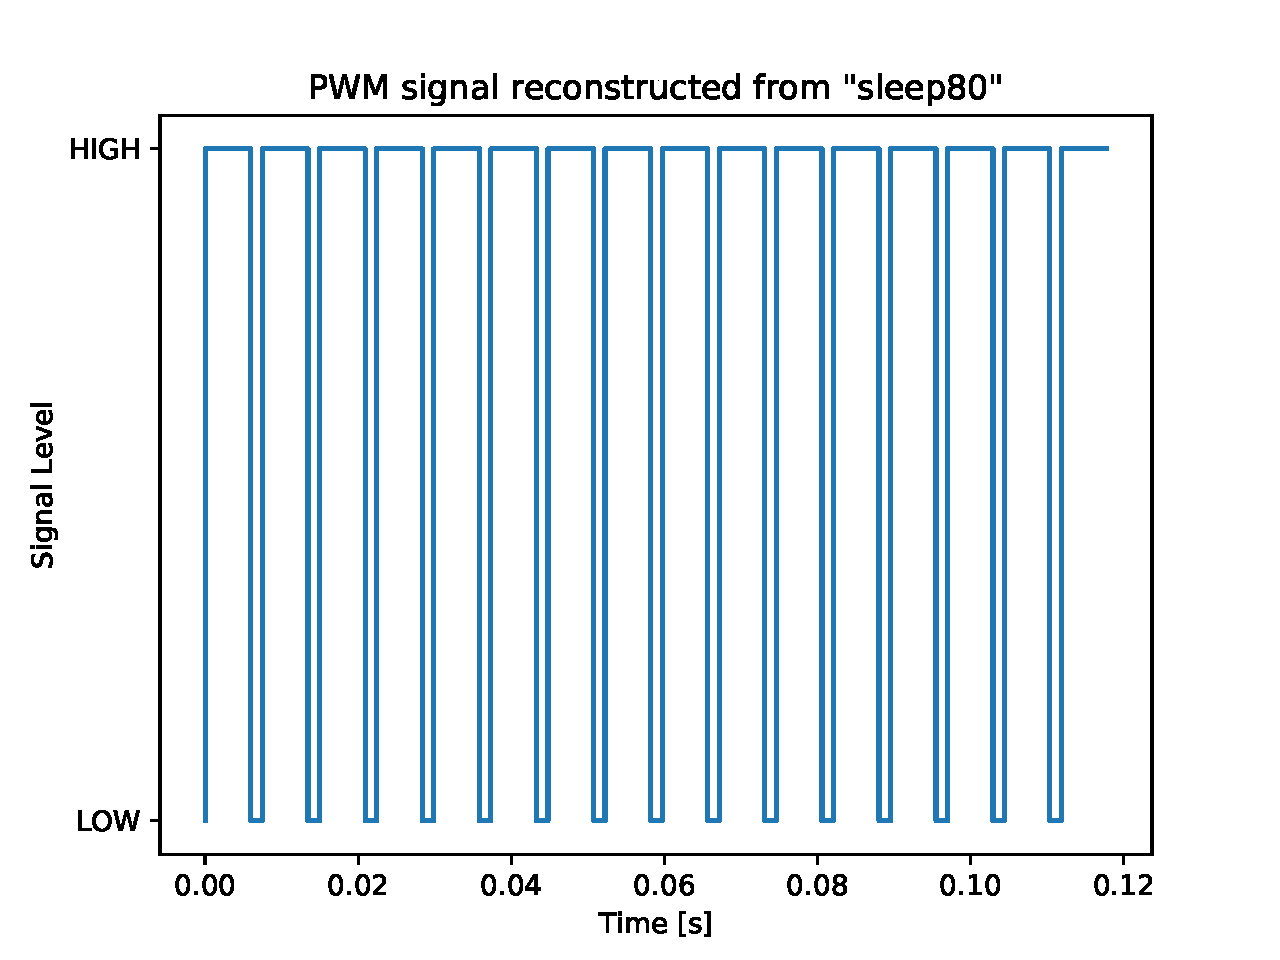
\includegraphics[width=\textwidth]{/home/schirner/work/ai-prog-workshop/presentation/images/edgeutil.png}
      \tiny\centerline{PWM signal}
    \end{column}
  \end{columns}

  \begin{alertbox}
    \begin{itemize}
      \item Students already overwhealmed with kernel module development
      \item Cannot ask to also write analysis code on top of everyting else
    \end{itemize}
  \end{alertbox}
\end{frame}

\begin{frame}[fragile]{Level 1 Example: Prompt and Output}
  \begin{columns}
    \begin{column}{0.6\textwidth}
    \begin{promptbox}
      The saved file is a comma separated file with the format outlined in the table below. All time stamps and durations are in seconds. Column Description 1 Sample Time 2 Edge type (0 for RISING, 1 for FALLING) 3 Duration since last edge of same type (e.g. RISING -> RISING) 4 Duration since last edge of opposite type (e.g. FALLING -> RISING). Plot cumulative probability of latency between falling and rising edge from this file.      
    \end{promptbox}
      \small\href{https://claude.ai/share/7e11fde4-bb5e-476e-b8f3-9dad820724f5}{Claude AI Session Link}
    \end{column}
    
    \begin{column}{0.4\textwidth}
      \begin{itemize}
        \item Generated: CSV read (\texttt{pandas}), CDF calculation (\texttt{numpy}), plot and save (\texttt{matplotlib})
        \item 110 lines of \href{https://github.com/neu-ece-esl/ai-prog-workshop/blob/main/1-script/analyze_latency.py}{Python Code}
      \end{itemize}
      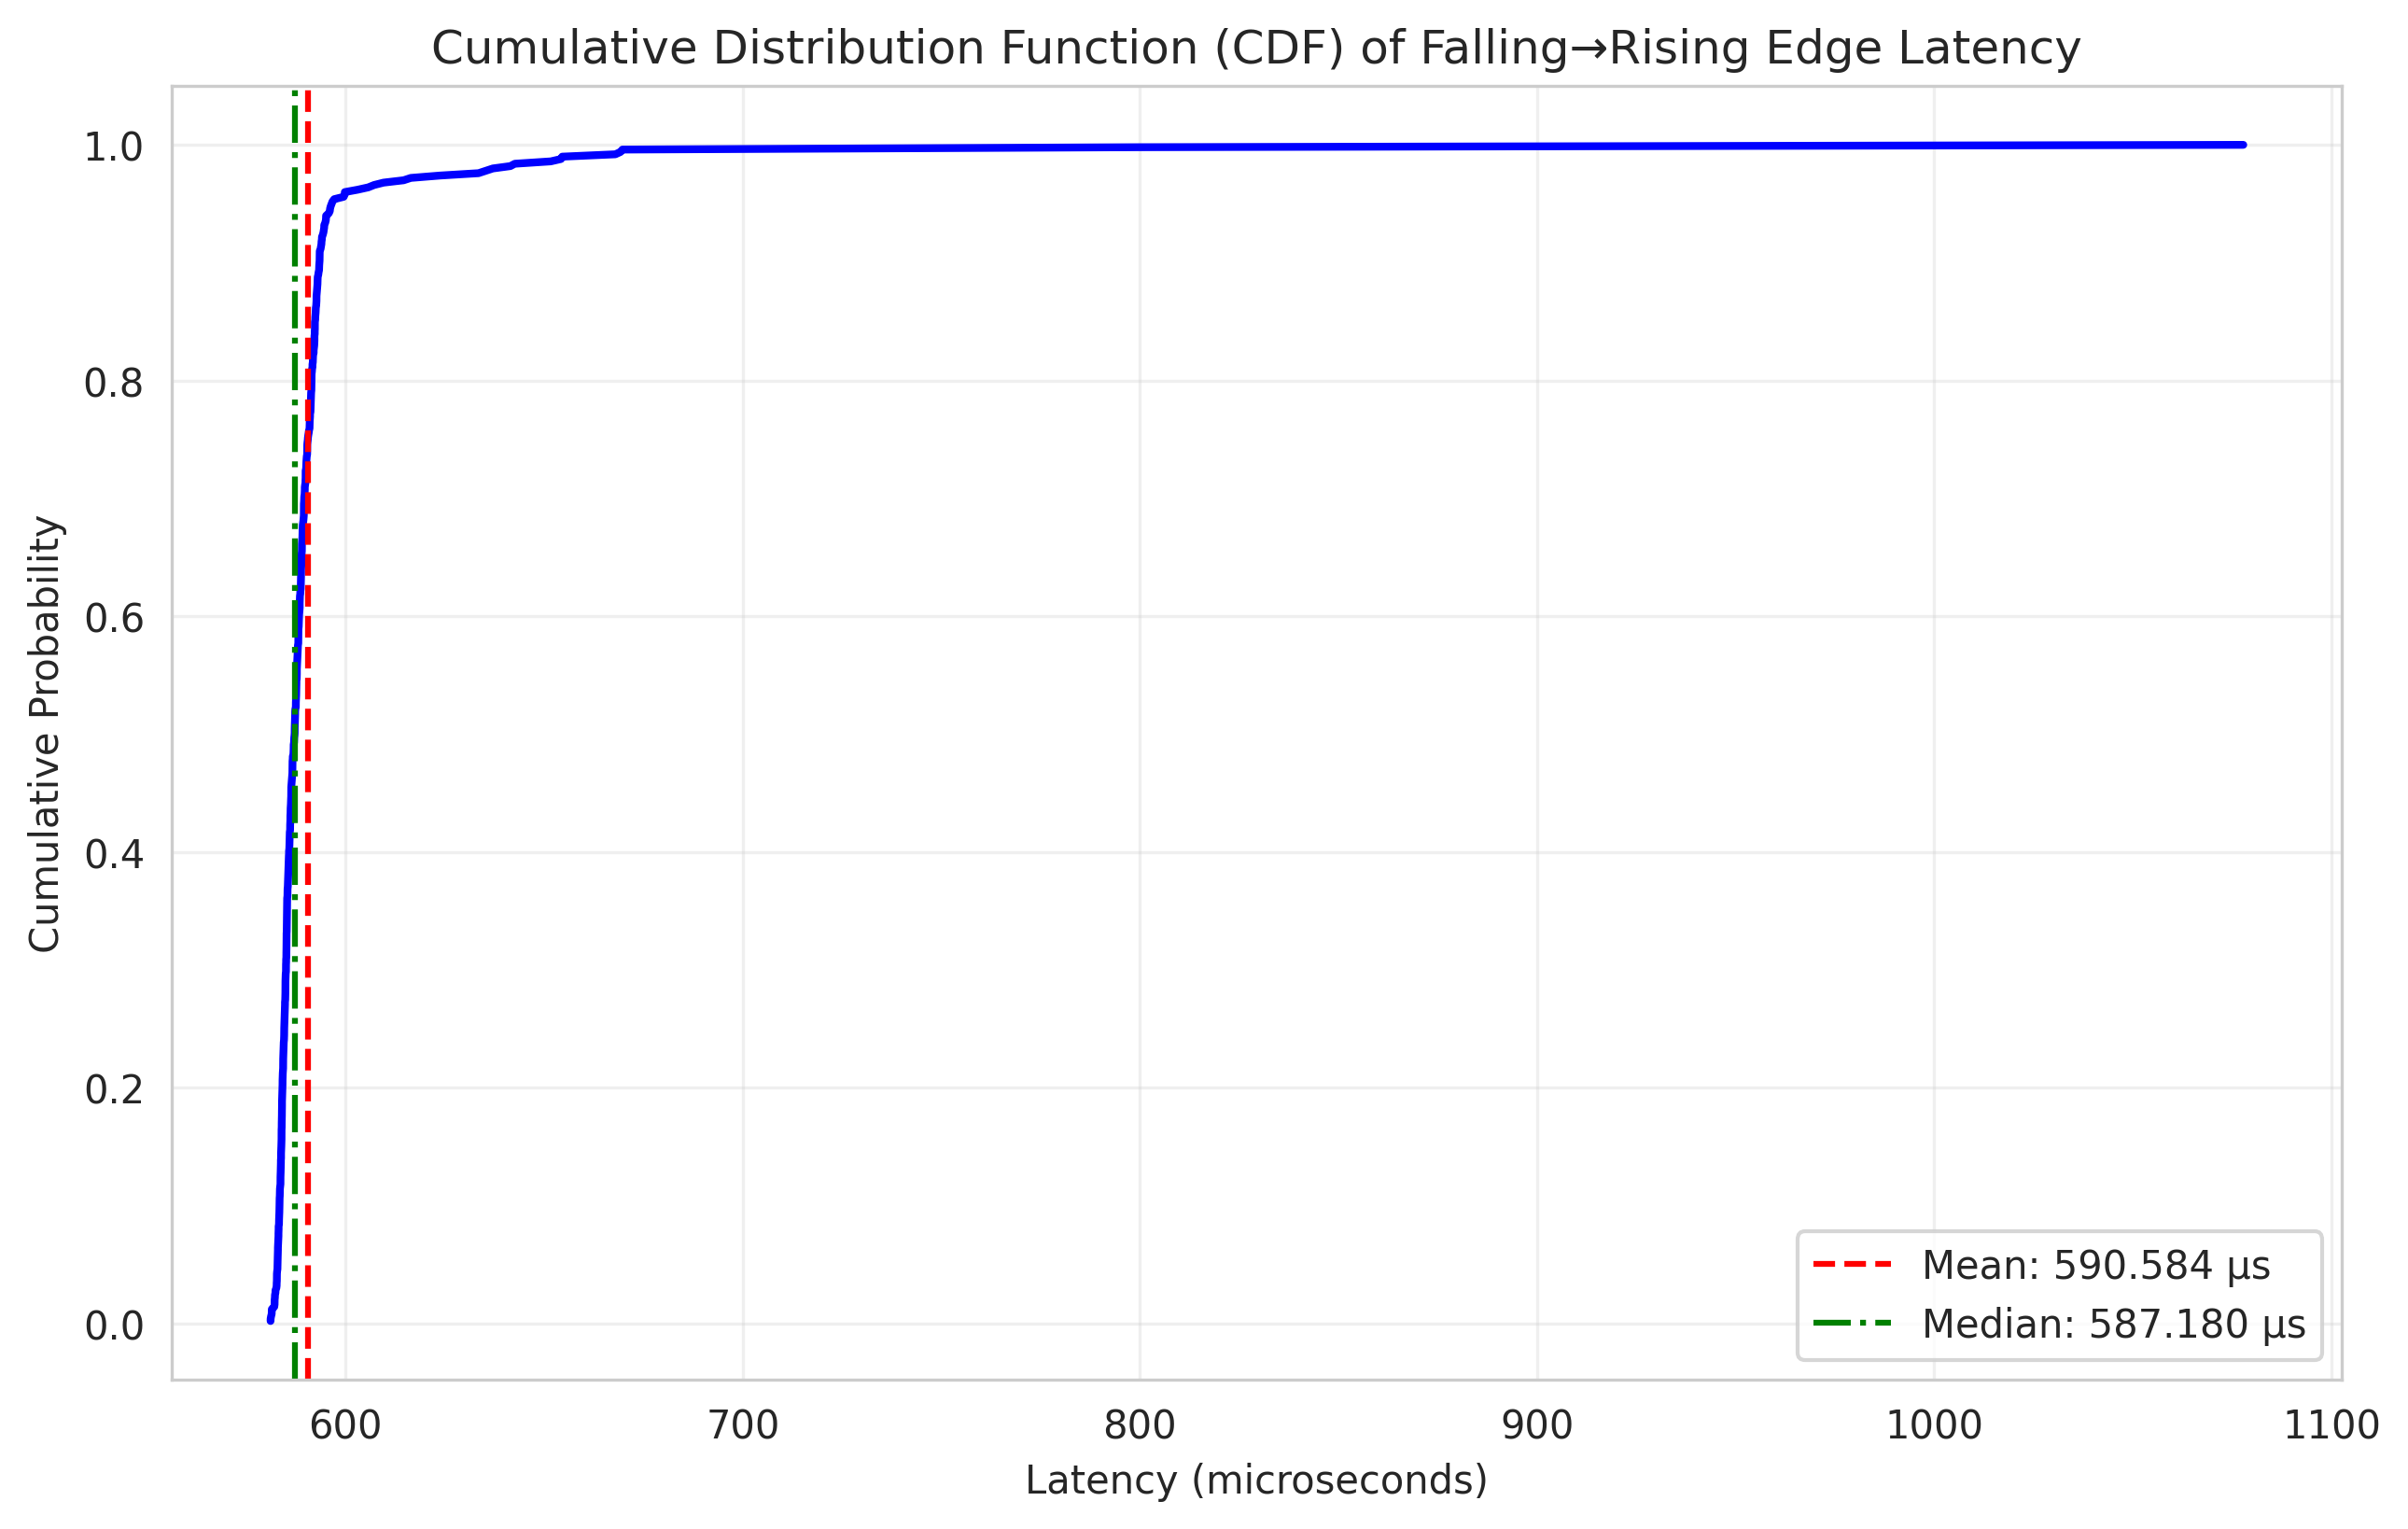
\includegraphics[width=\textwidth]{/home/schirner/work/ai-prog-workshop/1-script/pwm_sleep_edges_loaded_latency_cdf.png}
      \small\centerline{CDF of PWM Signal Latencies}
      
    \end{column}
  \end{columns}
\end{frame}

\begin{frame}{Level 1: Student Experience (Spring 2024)} 
    \begin{infobox}
    \begin{itemize}
        \item Excellent high-level discussion about real-time quality impact of
        \begin{itemize}
            \item Implementation method: busy loop, usleep, hardware timer
            \item Scheduling policy and priority 
            \item System load 
        \end{itemize}
    \end{itemize}
    \end{infobox}
    \begin{columns}
        \column{0.33\textwidth}
        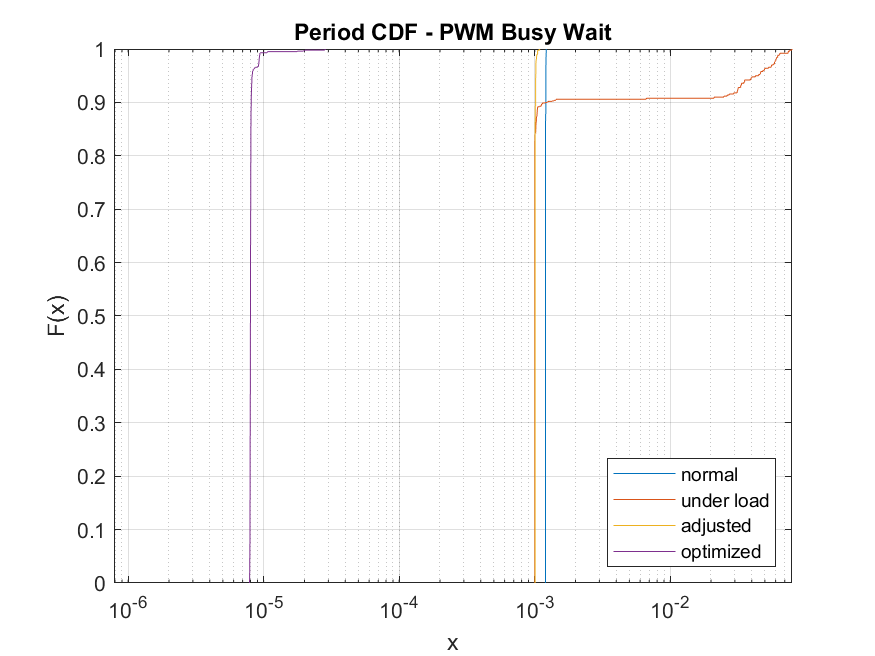
\includegraphics[width=\textwidth]{/home/schirner/work/ai-prog-workshop/1-script/period_busy.png}
        \tiny\centering (a) Busy Loop
        
        \column{0.33\textwidth}
        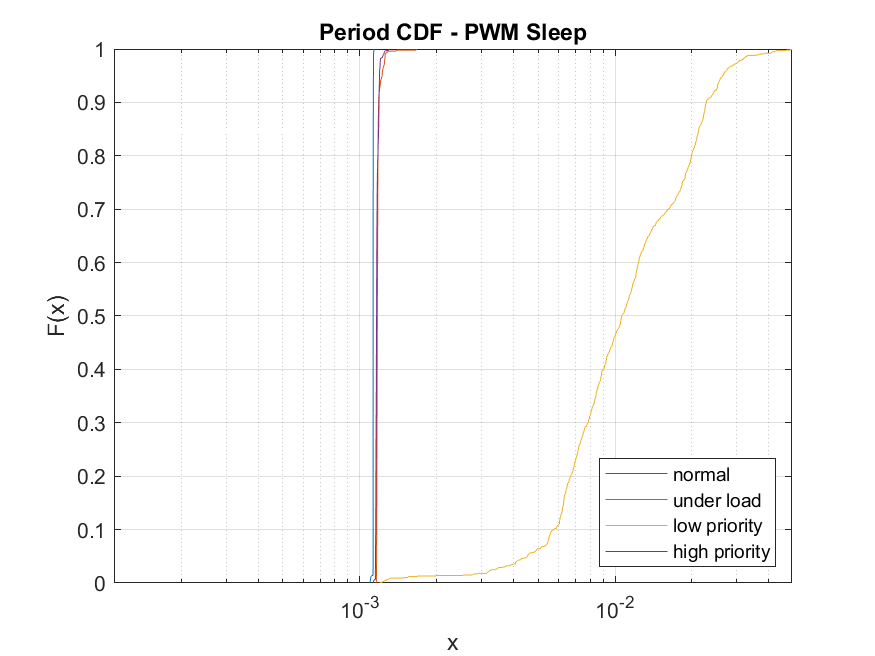
\includegraphics[width=\textwidth]{/home/schirner/work/ai-prog-workshop/1-script/period_sleep.png}
        \tiny\centering (b) OS Sleep
        
        \column{0.33\textwidth}
        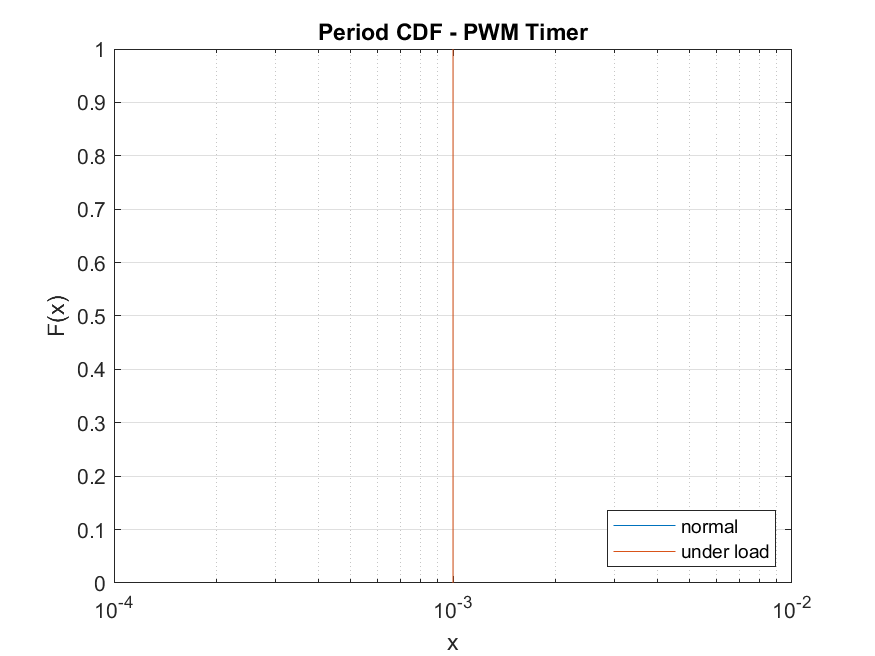
\includegraphics[width=\textwidth]{/home/schirner/work/ai-prog-workshop/1-script/period_timer.png}
        \tiny\centering (c) Hardware Timer
    \end{columns}
    \vspace{0.5em}
    \tiny For more details, see repo \href{https://github.com/neu-ece-esl/ai-prog-workshop/tree/main/1-script}{neu-ece-esl/ai-prog-workshop/1-script}.  
\end{frame}


\section{Level 2: Code Review and Improvement}

\begin{frame}{Level 2: Code Review and Improvement}

    \begin{columns}[T]
    \begin{column}{0.33\textwidth}
      \only<1->{\textbf{Pedagogical Need}
      \small The goal is not to let AI do the thinking for students, but to:
  \begin{itemize}
    \item Scaffold their problem-solving process
    \item Encourage students to first analyze code themselves
    \item Use AI for targeted hints or explanations
    \item Have students reflect on and evaluate AI's suggestions
  \end{itemize}
      }
    \end{column}
    
    \begin{column}{0.33\textwidth}
      \only<2->{\textbf{Technology Solution}
      \begin{itemize}\small
        \item Using AI as a coach to review, debug, and improve existing code
        \item Goal: Support student learning through hint-driven feedback
        \item Focuses on error identification and code optimization
        \item Provides guidance without directly giving away answers
      \end{itemize}
      }
    \end{column}
    
    \begin{column}{0.33\textwidth}
      \only<3->{\textbf{Benefits to Students}
    \begin{itemize}\small
      \item Deeper understanding of algorithms and logic
      \item Collaborative learning through discussion of AI output
      \item A mindset of \textit{debugging as discovery}, not just fixing
    \end{itemize}
      }
    \end{column}
  \end{columns}
  \vspace{0.5em}
  \tiny For more details, see repo \href{https://github.com/neu-ece-esl/ai-prog-workshop/tree/main/2-review}{neu-ece-esl/ai-prog-workshop/2-review}.  
\end{frame}

\begin{frame}[fragile]{Level 2: Example Merge Sort}
  \begin{columns}[T]
    \begin{column}{0.42\textwidth}
      After students attempt to understand and debug the code themselves:
      \begin{promptbox}
      %\begin{codeboxtc}{text}{AI Prompt}{}{linenos=false, frame=none, breaklines=false}
Can you review the following merge sort implementation and highlight any possible errors or inefficiencies? Please explain what is wrong, suggest corrections, and explain how the code can be made more efficient and robust.
      \end{promptbox}
      %\end{codeboxtc}
    \end{column}
    
    \begin{column}{0.52\textwidth}
      \vspace{-1.5em}
      \begin{codeboxtc}{python}{Faulty Merge Sort Implementation}{}{fontsize=\scriptsize}
    def merge_sort(arr):
        if len(arr) <= 1:
            return arr
        mid = len(arr) // 2
        left = merge_sort(arr[:mid])
        right = merge_sort(arr[mid]) 
        return merge(left, right)
    def merge(left, right):
        sorted_list = []
        i = j = 0
        while i < len(left) or j < len(right):          
            if i < len(left) and (j >= len(right) or left[i] < right[j]):
                sorted_list.append(left[i])
                i += 1
            else:
                sorted_list.append(right[j])
                j += 1
        return sorted_list\end{codeboxtc}
    \end{column}
  \end{columns}
\end{frame}

\begin{frame}[fragile]{Level 2 Example: Merge Sort Review}
  \begin{columns}[T]
    \begin{column}{0.42\textwidth}
      \begin{enumerate}
        \item \textbf{Incorrect Slice in Recursive Call}
          \begin{itemize}
            \item \texttt{right = merge\_sort(arr[mid])} should be \texttt{arr[mid:]}
          \end{itemize}
        
        \item \textbf{Unsafe Loop Condition}
          \begin{itemize}
            \item \texttt{while i < len(left) or j < len(right)} should use \texttt{and} to avoid \texttt{IndexError}
          \end{itemize}
        \item \textbf{Missing Appending of Remaining Elements}
          \begin{itemize}
            \item Any unprocessed elements in \texttt{left} or \texttt{right} should be appended after the loop
          \end{itemize}
      \end{enumerate}
    \end{column}
    
    \begin{column}{0.52\textwidth}
      \vspace{-1.5em}
      \begin{codeboxtc}{python}{Faulty Merge Sort Implementation}{}{fontsize=\scriptsize}
    def merge_sort(arr):
        if len(arr) <= 1:
            return arr
        mid = len(arr) // 2
        left = merge_sort(arr[:mid])
        right = merge_sort(arr[mid]) 
        return merge(left, right)
    def merge(left, right):
        sorted_list = []
        i = j = 0
        while i < len(left) or j < len(right):          
            if i < len(left) and (j >= len(right) or left[i] < right[j]):
                sorted_list.append(left[i])
                i += 1
            else:
                sorted_list.append(right[j])
                j += 1
        return sorted_list\end{codeboxtc}
    \end{column}
  \end{columns}
\end{frame}

\begin{frame}[fragile]{Level 2 Example: Merge Sort Corrected}
  \begin{columns}[T]
    \begin{column}{0.42\textwidth}
      After receiving AI's response, students should reflect on:
      \begin{itemize}
        \item Did the AI catch all the subtle bugs?
        \item Do they understand \textit{why} those bugs matter?
        \item Would students benefit from hint-driven support?
        \item What did they learn from this debugging process?
      \end{itemize}
    \end{column}
    
    \begin{column}{0.52\textwidth}
      \vspace{-1.5em}
      \begin{codeboxtc}{python}{Faulty Merge Sort Implementation}{}{fontsize=\scriptsize}
    def merge_sort(arr):
        if len(arr) <= 1:
            return arr
        mid = len(arr) // 2
        left = merge_sort(arr[:mid])
        right = merge_sort(arr[mid:])
        return merge(left, right)

    def merge(left, right):
        sorted_list = []
        i = j = 0
        while i < len(left) and j < len(right):
            if left[i] < right[j]:
                sorted_list.append(left[i])
                i += 1
            else:
                sorted_list.append(right[j])
                j += 1
        sorted_list.extend(left[i:])
        sorted_list.extend(right[j:])
        return sorted_list\end{codeboxtc}
    \end{column}
  \end{columns}
\end{frame}

\begin{frame}{Level 2 Code Review: Instructor Activity}
  Design a classroom activity where students use AI as a code reviewer:
  
  \begin{itemize}
    \item \textbf{What kind of faulty code will you use?}
      \begin{itemize}
        \item Algorithm with subtle logic bugs?
        \item Object-oriented implementation with structural issues?
        \item Larger codebase with inefficient logic?
      \end{itemize}
    \item \textbf{How will students interact with the AI?}
      \begin{itemize}
        \item To request hints or partial feedback?
        \item To compare their debugging with AI suggestions?
      \end{itemize}
  \end{itemize}
\end{frame}

\section{Level 3: Copilot Integration}

\begin{frame}{Level 3: Copilot in VS Code}
  \begin{columns}[T]
    \begin{column}{0.33\textwidth}
      \only<1->{\textbf{Pedagogical Need}
      \begin{itemize}\small
        \item Implementing the \textit{right} way is effort
        \begin{itemize}\footnotesize
          \item Refactoring for object-oriented design, readability, and maintainability  
          \item Test harnessing
          \item Data loaders to deal with large datasets
        \end{itemize}
        \item Students need to focus on design and intent
      \end{itemize}}
    \end{column}

%  GitHub Copilot isn't just a shortcut—it's a design collaboration tool:
%  \begin{itemize}
%    \item Helps translate high-level \textbf{intent} into functional code
%    \item Encourages focus on solution \textbf{design} rather than syntax
%    \item Shifts emphasis from "getting code to run" to:
%      \begin{itemize}
%        \item \textbf{Designing} robust, readable, purposeful code
%        \item Reviewing suggestions to ensure alignment with intent
%        \item Making \textbf{critical decisions} about accepting, rejecting, or revising completions
%      \end{itemize}
%  \end{itemize}   

    \begin{column}{0.33\textwidth}
      \only<2->{\textbf{Technology Solution}
      \begin{itemize}\small
        \item GitHub Copilot as a coding assistant in VS Code
        \item Provides context-aware code completions and suggestions
        \item Generates boilerplate code and scaffolds structures from natural language
      \end{itemize}}
    \end{column}
    
    \begin{column}{0.33\textwidth}
      \only<3->{\textbf{Benefits to Students}
      \begin{itemize}\small
        \item Helps students focus on higher-level design thinking
        \item Reduces cognitive load of syntax and boilerplate
        \begin{itemize}\footnotesize
          \item Creates room to encourage proper SW design and testing setup
        \end{itemize}
        \item Facilitates deeper engagement with programming concepts
        \item Encourages critical evaluation of AI-generated suggestions
      \end{itemize}}
    \end{column}
  \end{columns}
\end{frame}


\begin{frame}{Level 3 Example: Cluster Visualization}
  \begin{columns}
    \begin{column}{0.6\textwidth}
      \begin{itemize}
        \item Task: KMeans clustering of customer data
        \item Students analyze and visualize clustering results
        \item AI-generated code for data loading, preprocessing, and visualization
      \end{itemize}
      \vspace{0.5em}
      \href{https://github.com/neu-ece-esl/ai-prog-workshop/tree/main/3-assist}{Link to Animation: GitHub Copilot completing code}
      \vspace{0.5em}
      \begin{itemize}
        \item Well-structured comments guide Copilot suggestions
        \item Examples of functions Copilot can generate:
        \begin{itemize}
          \item \texttt{plot\_cluster\_distribution()}
          \item \texttt{evaluate\_clustering\_quality()}
        \end{itemize}
      \end{itemize}
    \end{column}
    
    \begin{column}{0.4\textwidth}
      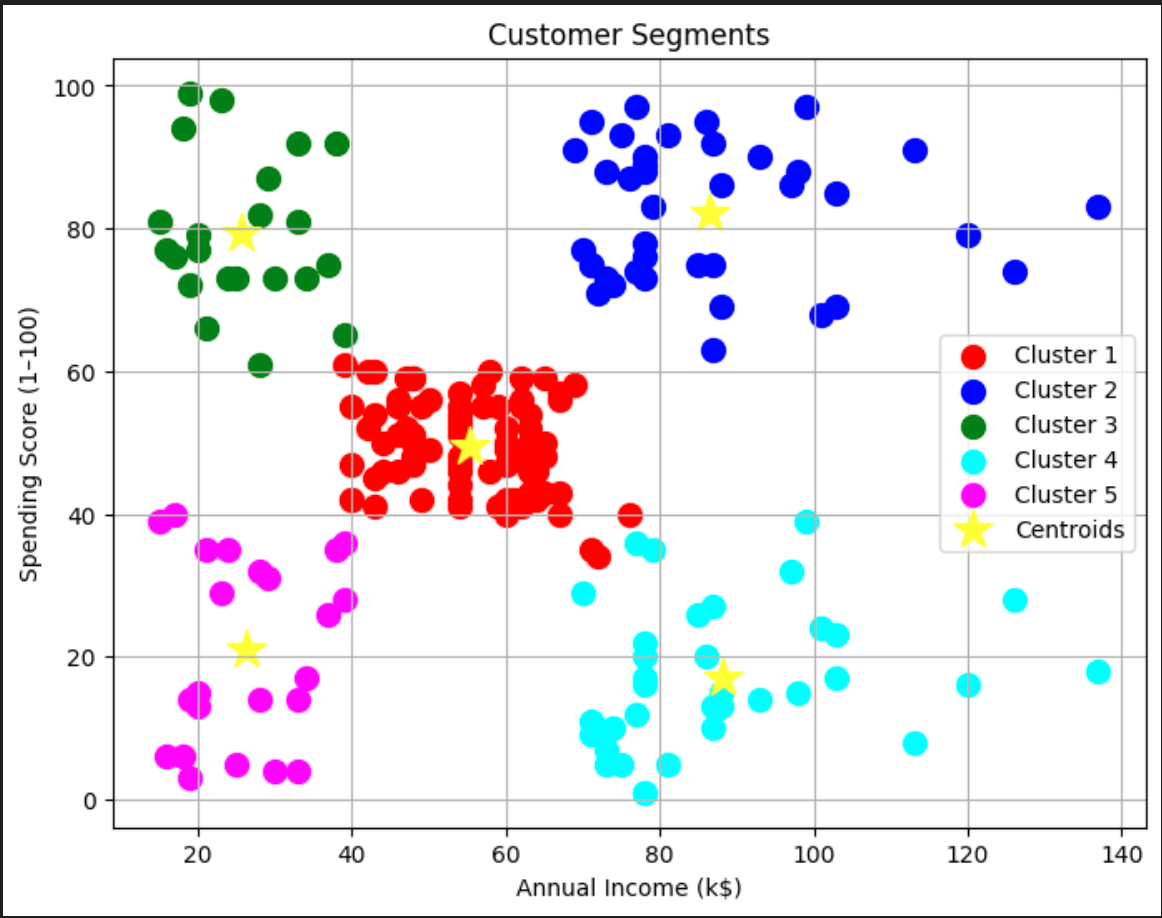
\includegraphics[width=0.9\textwidth]{/home/schirner/work/ai-prog-workshop/3-assist/Cluster.jpeg}
      \tiny\centerline{Image: K-Means clustering of customer data}
      \tiny\centerline{\href{https://github.com/neu-ece-esl/ai-prog-workshop/blob/main/3-assist/KMeans_Clustering.ipynb}{Jupyter Notebook}}

      \begin{itemize}
        \item Scatter plot showing KMeans clustering of customers
        \item Based on annual income and spending score
        \item Students might analyze or reproduce such results
      \end{itemize}
    \end{column}
  \end{columns}
\end{frame}


\begin{frame}{Level 3 Assist: Instructor Activity: Copilot Integration}
  Design a classroom activity where students:
  \begin{enumerate}
    \item Start from a partially written script or data processing task
    \item Use Copilot to complete functions, generate visualizations, or structure test code
    \item Reflect on how closely Copilot's output matches their original design intent
  \end{enumerate}
  
  Consider:
  \begin{itemize}
    \item What prompt would you give your students?
    \item How would you ensure critical evaluation of suggestions?
    \item Could this accelerate exploration of real-world datasets?
  \end{itemize}
\end{frame}

\section{Level 4: Agent Mode for Complex Projects}

\begin{frame}{Level 4: Agent Mode for Complex Projects}
  \begin{columns}[T]
    \begin{column}{0.33\textwidth}
      \only<1->{\textbf{Pedagogical Need}
      \begin{itemize}\small
        \item Experiential learning is key, involving hands-on final projects
        \item Class projects are time-constrained (4-6 weeks), limiting scope
        \item Opportunity: increase impact using Agent Mode for development
      \end{itemize}}
    \end{column}
    
    \begin{column}{0.33\textwidth}
      \only<2->{\textbf{Technology Solution}
      \begin{itemize}\small
        \item Using GitHub Copilot Agent Mode to tackle complex, multi-file projects
        \item Simple prompts can generate entire codebases
        \item Manages sophisticated projects that would be challenging in classroom contexts
      \end{itemize}}
    \end{column}
    
    \begin{column}{0.33\textwidth}
      \only<3->{\textbf{Benefits to Students}
      \begin{itemize}\small
        \item Focus on system architecture and design principles
        \item Tackle more ambitious, real-world projects
        \item Develop system thinking while reducing implementation overhead
        \item Enables ambitious projects that demonstrate real-world scenarios
        \item More experiential learning in less time
      \end{itemize}}
    \end{column}
  \end{columns}
\end{frame}

\begin{frame}{Level 4: Vibe Coding}
  \begin{tcolorbox}[colback=green!10!white, colframe=green!60!black, title=Vibe Coding]
    \begin{itemize}
      \item Focuses on rapid prototyping and collaborative iteration with AI
      \item Prioritizes agile evolution of user experience and system flow over low-level details
      \item Enables quick project scaffolding and experimentation
      \item Mainstream in startups and accelerators:
        \begin{itemize}\footnotesize
          \item 25\% of Y Combinator's current cohort have almost entirely AI-generated codebases
        \end{itemize}
    \end{itemize}
  \end{tcolorbox}
  \begin{tcolorbox}[colback=red!10!white, colframe=red!60!black, title=Challenges]
    \begin{itemize}
      \item Students still need to understand the entire stack
      \item Must critically evaluate AI suggestions and spot issues
      \item Large volume of generated code can become overwhelming
      \item Need to balance convenience with learning goals
    \end{itemize}
  \end{tcolorbox}
\end{frame}

\begin{frame}{Level 4 Example: HW / SW Co-design Project} 
    \centering EECE7368 Hardware/Software Co-design Fall 2024 (\href{https://neu-ece-7368.github.io/}{page})   \begin{columns}[T]
    \begin{column}{0.4\textwidth}
      \begin{itemize}
        \item Accelerate AI inference with GEMM Accelerator 
        \begin{itemize}
          \item SoC and custom hardware simulation
          \item Focus on HW/SW architecture
        \end{itemize}
        \item Very deep technology stack
        \begin{itemize}\footnotesize
            \item \href{https://www.qemu.org/}{QEMU} simulating ARM CPU w/Linux OS
            \item Custom GEMM accelerator in \href{https://systemc.org/}{SystemC} (C++ library extension)
            \item Custom register interface to expose accelerator to CPU 
            \item User space driver for interfacing with own GEMM accelerator
            \item AI inference engine in C \href{https://github.com/pjreddie/darknet}{darknet}
          \end{itemize}
      \end{itemize}
    \end{column}
    \begin{column}{0.6\textwidth}
      \hfill 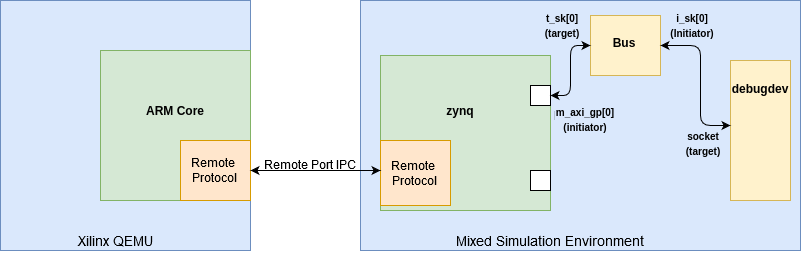
\includegraphics[width=0.9\textwidth]{images/QemuCosim.png}
      \tiny\centerline{Image: QEMU Co-simulation of ARM CPU and GEMM Accelerator}

      \begin{alertbox}
        Fall 2024: While allowed to use any AI, anythying available. Students did work mostly manually. 
      \end{alertbox}
    \end{column}
  \end{columns}
\end{frame}

\begin{frame}{Level 4 Example: Group Organization Tool}
  \begin{columns}
    \begin{column}{0.5\textwidth}
      \begin{itemize}
        \item Organizing workshop participants into groups based on interests
        \item Complex web application, requires full stack development knowledge
        \item Too much, too difficult.
        \item Can AI get it done?
      \end{itemize}
    \end{column}
    
    \begin{column}{0.5\textwidth}
      \begin{promptbox}\footnotesize
        Generate a web page to which session participants can login (just by name no authentication required). After logging in, each participant needs to select from one of the following interests:
        \begin{itemize}\vspace{-0.5em}
          \item Code Improvement and Teaching
          \vspace{-0.5em}
          \item Code Assistance with CoPilot
          \vspace{-0.5em}
          \item Script Generation
          \vspace{-0.5em}
          \item Agent Mode for Projects
          \vspace{-0.5em}
       \end{itemize}
A coordinator (username admin) finishes the first phase (after all participants have logged in). Then participants are paired together based on interests into teams (Teams get named team-1, team-2 ...). Each team should contain 2-2 members. The participants should get their team name and team members displayed once the decision is done. Optionally, members in the tam should be able to chat with each other
      \end{promptbox}
    \end{column}
  \end{columns}
\end{frame}

\begin{frame}{Level 4 Example: Group Organization Tool 2}
  \begin{columns}[T]
    \begin{column}{0.5\textwidth}
      \begin{itemize}
          \item Generated NPM javascript web application (I have no idea)
          \item Application almost works out of the box
      \end{itemize}
      \begin{alertbox}\small
          Phase 2: of notifying participants of their group did \textbf{not} work
      \end{alertbox}
      \begin{promptbox}\small
        The website worked and participants could login an dstate interests. However, once the admin as selected "form teams" it gets the message "teams sucessfully formed" but the participants still see the status "waiting for team forming"
      \end{promptbox}
    \end{column}
    \begin{column}{0.5\textwidth}
        
      \centering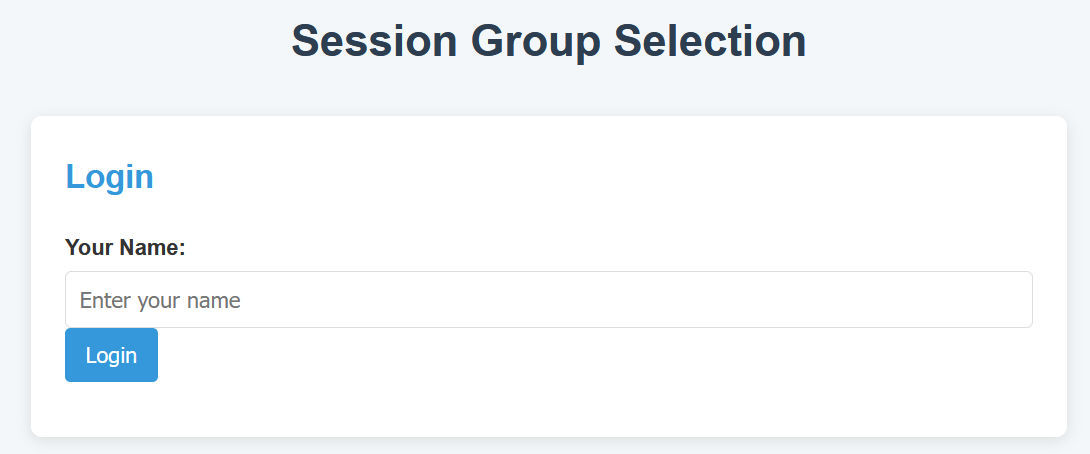
\includegraphics[width=0.7\textwidth]{images/GroupOrg.png}
      \tiny\centerline{Image: Login Page}
      \centering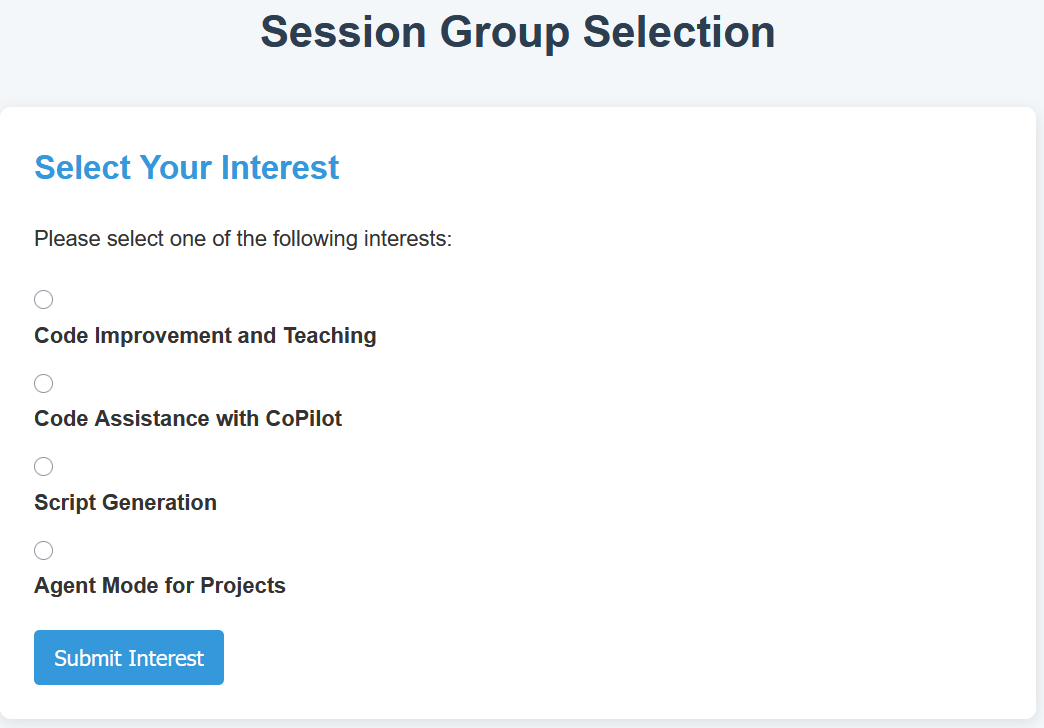
\includegraphics[width=0.7\textwidth]{images/GroupOrg2.png}
      \tiny\centerline{Image: Interest Selection}
    \end{column}
  \end{columns}
\end{frame}

\begin{frame}{Level 4 Example: Group Organization Tool (Reflection)}
\begin{itemize}
  \item App generation demonstrates technical capabilities, but lacks pedagogical framing.
  \item No learning involved; the domain is outside my expertise, making it difficult to digest and evaluate the generated code.
  \item No reflection on the process or outcomes.
  \item Technical gaps remain, such as missing HTTPS and deploying code without review.
\end{itemize}

\begin{alertbox}
\begin{itemize}
  \item How to drive pedagogical value from this tech capability? 
  \item Let's discover together.
\end{itemize}  
\end{alertbox}
\end{frame}

\begin{frame}{Instructor Activity: Agent Mode}
  Consider how you might use Agent Mode in your teaching:
  
  \begin{enumerate}
    \item Identify a complex, multi-component project that would normally be challenging to implement
    \item Draft a detailed system specification focusing on learning objectives
    \item Create a prompt template for students to use with Agent Mode
    \item Consider assessment criteria emphasizing system design, integration patterns, and architectural choices
  \end{enumerate}
  
  This approach allows students to engage with sophisticated projects while developing valuable system thinking skills.
\end{frame}

\part[Hands-on Activity]{Hands-on Activity}
\section{Activity Design}

\begin{frame}{Hands-on Activity Overview}
  Form groups of 2 based on interest in AI assistance levels:
  \begin{itemize}
    \item Preferably select a level challenging you beyond current experience
    \item Your team will be assigned a breakout room
  \end{itemize}
  
  Then:
  \begin{itemize}
    \item Explore your chosen technology level
    \item Design a classroom activity integrating AI at this level
    \item Leverage AI assistants to build your activity
    \item Prepare to share with the larger group
  \end{itemize}
  
  Time: 15 minutes
\end{frame}

\begin{frame}{Activity Design Considerations}
  When designing your activity, consider:
  \begin{itemize}
    \item Expected outcomes/skills
    \item Expressiveness and scalability of assessment
    \item How to minimize anticipated challenges
    \item Ways to foster student engagement and ownership
    \item Opportunities for deeper learning
  \end{itemize}
\end{frame}

\part[Discussion and Reflection]{Discussion and Reflection}
\section{Show \& Tell}

\begin{frame}{Share and Discuss}
  \begin{itemize}
    \item Selected groups share activity ideas, challenges, and insights
    \item Discuss implementation approaches
    \item Identify common themes and innovations
    \item Consider adaptations for different course contexts
  \end{itemize}
\end{frame}

\section{Reflection}

\begin{frame}{Impact on Learning}
  \begin{itemize}
    \item Discuss how integrating AI could impact student learning
    \item Consider ways tools might reshape assignments and course design
    \item Identify potential challenges in:
      \begin{itemize}
        \item Assessment
        \item Fairness
        \item Over-reliance on AI
      \end{itemize}
    \item Explore opportunities to foster deeper engagement and ownership
  \end{itemize}
\end{frame}

\begin{frame}{Continued Exploration}
  \begin{itemize}
    \item Too many ideas, too many changes to explore in one hour!
    \item Launchpad for ongoing discussion and collaboration
    \item Consider regular (e.g., bi-weekly) meetups to:
      \begin{itemize}
        \item Share observations, challenges, and new ideas
        \item Support each other in programming education evolution
      \end{itemize}
    \item Next step: kick-off programming community meeting
  \end{itemize}
\end{frame}

\part[Conclusion]{Conclusion}
\section{Conclusion}

\begin{frame}{Contributing \& Continuing the Conversation}
  We welcome contributions from instructors adapting these resources:
  \begin{itemize}
    \item Fork the repository and customize materials
    \item Submit issues or suggestions for improvement
    \item Add your own classroom AI integration examples
  \end{itemize}
  
  Let's build a collaborative, forward-thinking community of educators who embrace AI not as a shortcut—but as a tool for thoughtful, empowering, and meaningful learning.
\end{frame}

\begin{frame}{Acknowledgments}
  This workshop was created by:
  \begin{itemize}
    \item \href{https://coe.northeastern.edu/people/schirner-gunar/}{Gunar Schirner}
    \item \href{https://coe.northeastern.edu/people/nafa-fatema/}{Fatema Nafa}
    \item Muhammad Salman
  \end{itemize}
  
  at Northeastern University.
  
  \vspace{1em}
  
  Claude and other AI tools have been used in the process of ideation and drafting the workshop.
\end{frame}

\begin{frame}{Thank You!}
  \begin{center}
    \Large{Questions and Discussion}
    
    \vspace{2em}
    
    GitHub Repository:\\
    \texttt{https://github.com/neu-ece-esl/ai-prog-workshop}
  \end{center}
\end{frame}

\end{document}
